\documentclass{article}
\usepackage{amsmath,amssymb,graphicx,hyperref,booktabs,float,subcaption}
\usepackage[margin=1in]{geometry}

\begin{document}

\tableofcontents	

\section{Executive Summary}

\section{Clustering and Dimensionality Reduction}
In this section we outline the process and results of applying the K-Means Clustering algorithm, and the Principal Component Analysis (PCA) and the Uniform Manifold Approximation and Projection (UMAP) dimensionality reduction techniques to learn if there are segments or axes of grouping in our data that allow us to uncover meaningful patterns or characteristics and guide subsequent predictive modeling.

\subsubsection{Data Preprocessing}

To prepare the data for clustering and dimensionality reduction, we performed a series of preprocessing steps to ensure data quality, remove information leakage, and align features for unsupervised learning.

First, we merged the DemoStats and HouseholdSpend datasets on their common Dissemination Area (DA) identifiers. We removed the DA identifier columns post-merge, as they are non-informative for clustering and dimensionality reduction.

Next, we addressed missing data. We identified a set of variables with over 10\% missingness, many related to median age attributes (e.g., median age of mothers at first birth, median age of female maintainers). Despite the missingness, these features demonstrated non-negligible correlations with the target variable. To preserve their potential explanatory power without introducing bias, we imputed missing values using the median of each column.

To prevent data leakage into the clustering process, we dropped variables directly or indirectly tied to the target variable. This included any column names containing keywords such as ‘income’, ‘insurance’, ‘pension’, ‘retirement’, and ‘tax’, resulting in the removal of 47 features. This ensured that the clusters would not be shaped by information that directly influences our regression target.

Outlier treatment was a key step due to the highly skewed nature of the dataset. We applied IQR-based winsorization, replacing values beyond 1.5 times the interquartile range at the respective thresholds with their respective boundary values. We preferred this method over z-score based outlier replacement, as z-scores internalize the distribution’s skewness, potentially skewing results even further in long-tailed features.

Finally, we standardized the dataset using z-score normalization. Since both K-Means and PCA are sensitive to feature scales, this step ensures equal weighting across all variables.

These preprocessing steps yielded a refined dataset ready for clustering and dimensionality reduction, with reduced noise, consistent scaling, and mitigated risk of information leakage.

\subsubsection{K-Means Clustering}

Given the size of the dataset, we applied the Elbow and Silhouette methods on a 10\% random sample of the data to identify a suitable number of clusters for K-Means. This approach balanced computational efficiency with reliable estimation of clustering structure.

The Elbow method (Figure~\ref{fig:elbow}) shows a noticeable change in the distortion score curve at $k=4$, suggesting that four clusters strike a good balance between model complexity and explained variance.

\begin{figure}[H]
    \centering
    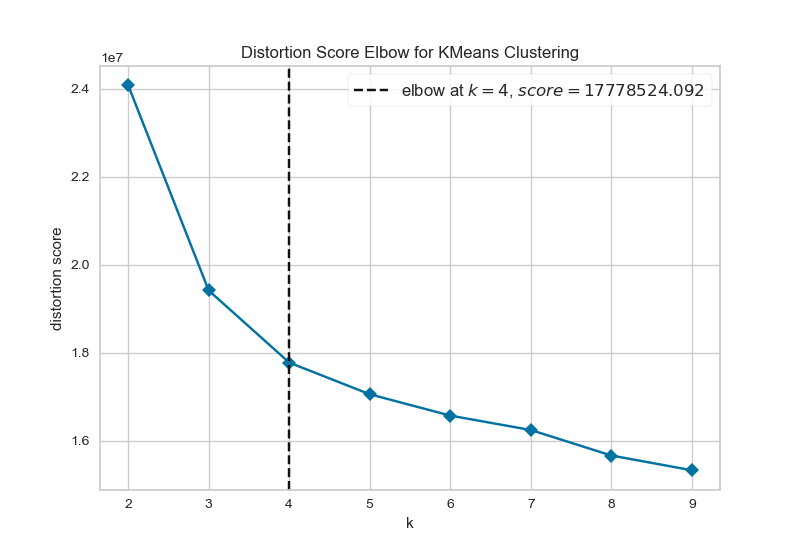
\includegraphics[width=0.7\textwidth]{figures/elbow_plot.png}
    \caption{Distortion Score Elbow for KMeans Clustering}
    \label{fig:elbow}
\end{figure}

To complement this, we examined the Silhouette scores for $k=2$, $k=3$, and $k=4$ in Figures~\ref{fig:silhouette_k2}, \ref{fig:silhouette_k3}, and \ref{fig:silhouette_k4}. The plots illustrate a trade-off between cohesion and interpretability. At $k=2$ (Figure~\ref{fig:silhouette_k2}), the average Silhouette score is highest, indicating strong separation between clusters, though the result may be overly coarse. At $k=3$ (Figure~\ref{fig:silhouette_k3}), a more interpretable clustering appears with moderate cohesion. At $k=4$ (Figure~\ref{fig:silhouette_k4}), the score drops further, and clusters begin to overlap more significantly.

\begin{figure}[H]
    \centering
    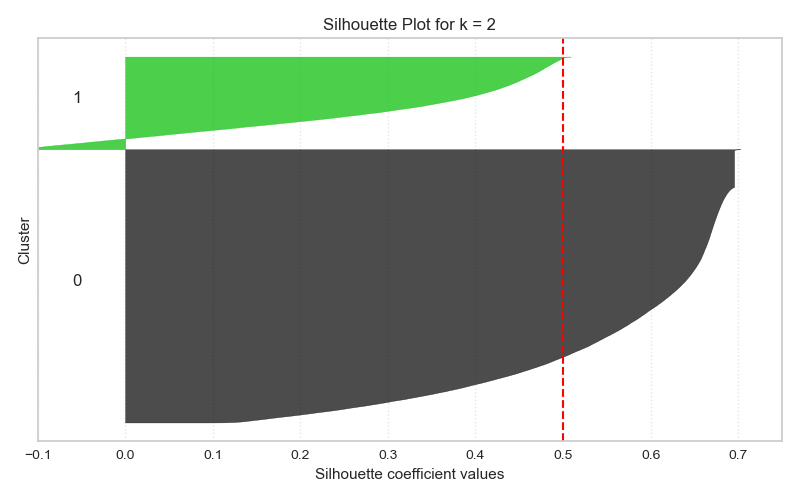
\includegraphics[width=0.6\textwidth]{figures/silhouette_k2.png}
    \caption{Silhouette Plot for $k=2$}
    \label{fig:silhouette_k2}
\end{figure}

\begin{figure}[H]
    \centering
    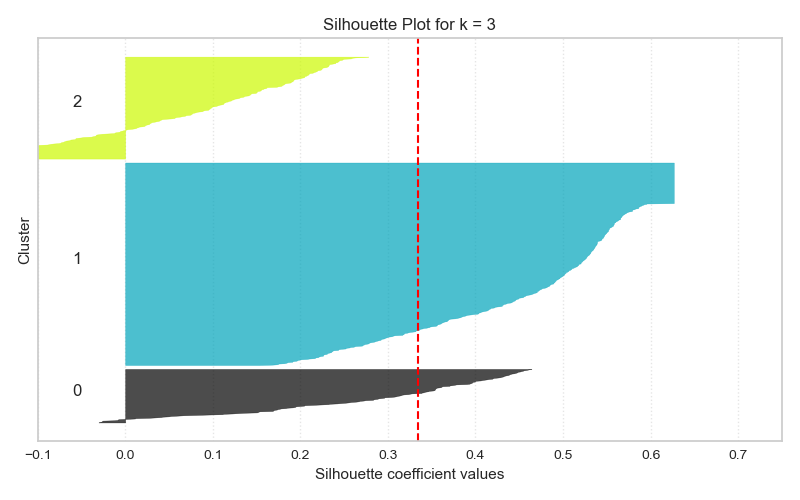
\includegraphics[width=0.6\textwidth]{figures/silhouette_k3.png}
    \caption{Silhouette Plot for $k=3$}
    \label{fig:silhouette_k3}
\end{figure}

\begin{figure}[H]
    \centering
    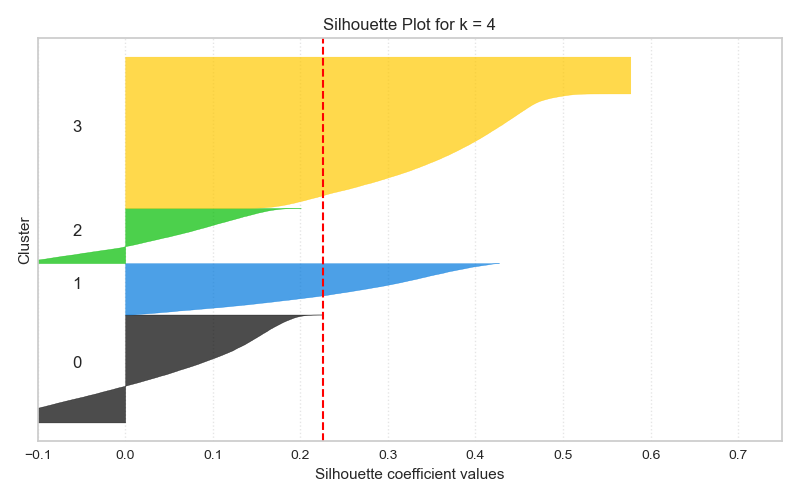
\includegraphics[width=0.6\textwidth]{figures/silhouette_k4.png}
    \caption{Silhouette Plot for $k=4$}
    \label{fig:silhouette_k4}
\end{figure}

The Silhouette plot for $k=5$ (Figure~\ref{fig:silhouette_k5}) and a comparison of average Silhouette scores across $k=2$ to $k=5$ (Figure~\ref{fig:silhouette_scores}) are included in the appendix and referenced here to further support our choice of $k=3$.

Overall, both the Elbow and Silhouette methods suggest $k=2$ and $k=3$ as viable options. The clearer cluster structure observed at $k=3$ combined with interpretability benefits, led us to select $k=3$ as the final number of clusters. These labels were retained for subsequent dimensionality reduction and interpretation.


\subsubsection{Principal Component Analysis}

To explore latent structure in the data, we applied Principal Component Analysis (PCA), a linear dimensionality reduction technique. We compared results on both unscaled and standardized data. Although PCA on unscaled data yielded a first component that explains 98.8\% of the variance, this result was driven largely by the presence of features with larger numeric scales. In contrast, the scaled version, where all variables are z-score normalized, produced a more balanced set of principal components, with the first three PCs explaining 67.9\%, 3.7\%, and 3.0\% of the variance, respectively. Therefore, all PCA analyses moving forward are based on the scaled data.

Figure~\ref{fig:pca3d} illustrates 3D scatterplots of the first three principal components for both the unscaled and scaled data, coloured by the K-Means cluster labels ($k=3$). The scaled data plot reveals broad, loosely separated regions aligned with the cluster assignments, though some overlap remains, suggesting that the clustering structure is not sharply defined but does capture some underlying gradients in the data.

\begin{figure}[H]
    \centering
    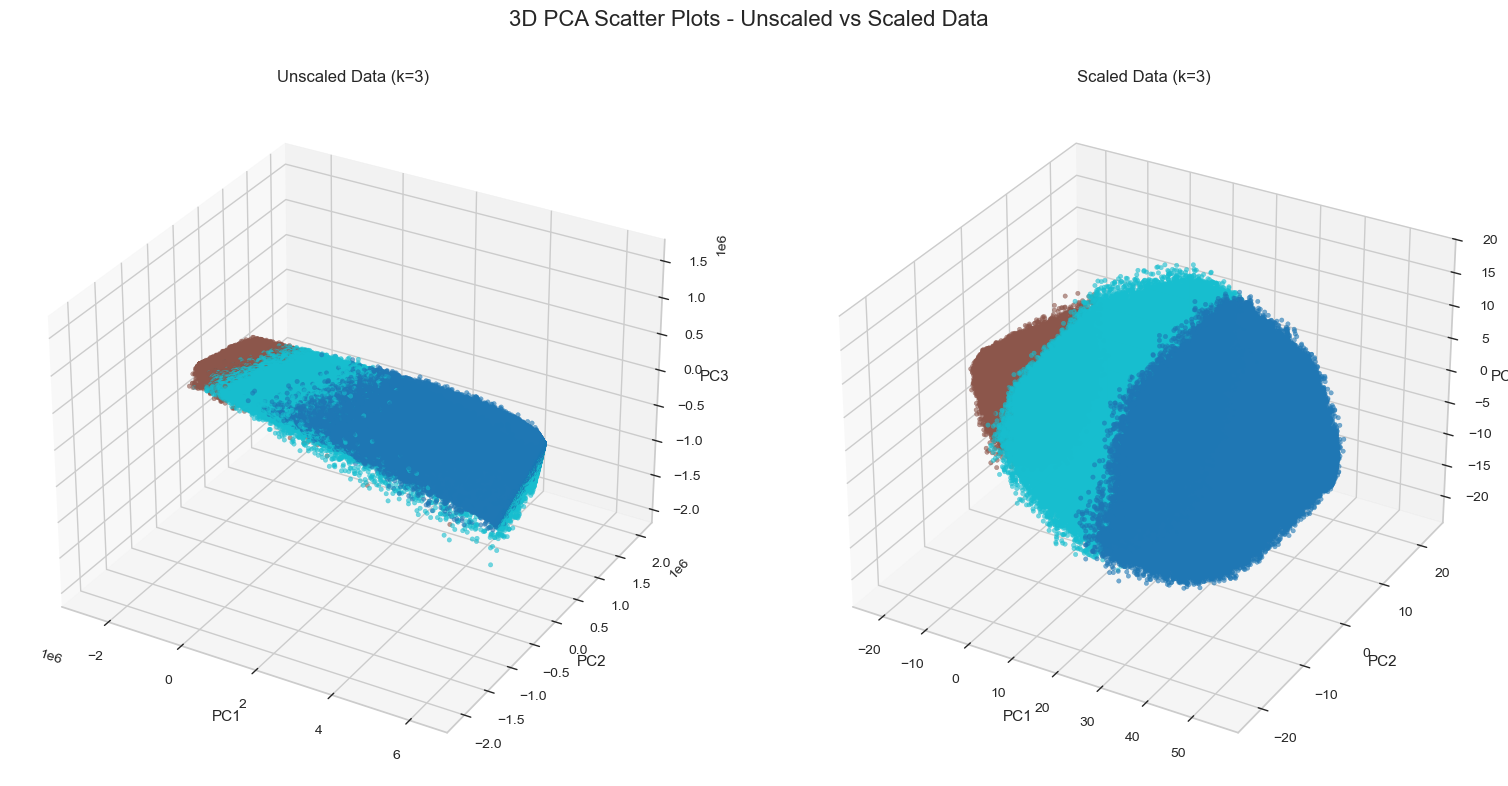
\includegraphics[width=\textwidth]{figures/pca3d_scaled_vs_unscaled.png}
    \caption{3D PCA Scatter Plots Comparing Unscaled (Left) vs. Scaled (Right) Data}
    \label{fig:pca3d}
\end{figure}

We calculated the top five positive and negative contributors to each of the first three principal components and grouped them by variable category for interpretability. The detailed variable-level contributions are presented in Appendix Tables~\ref{tab:pc1_pos}--\ref{tab:pc3_neg}.

\paragraph{PC1: Economic Activity and Household Presence.}  
PC1 appears to capture a dimension tied to household economic activity and consumer behavior. The dominant contribution from the \textit{Consumption} category (Figure~\ref{fig:pc1}) suggests that higher PC1 scores are associated with greater household spending. This is supported by additional contributions from population-related categories like \textit{Total Household Population by Age}, indicating these are also demographically dense areas. Contributions from \textit{Household Population 15+ by Industry} further reinforce the interpretation that PC1 reflects regions with economically active residents and a strong consumer presence.

\begin{figure}[H]
    \centering
    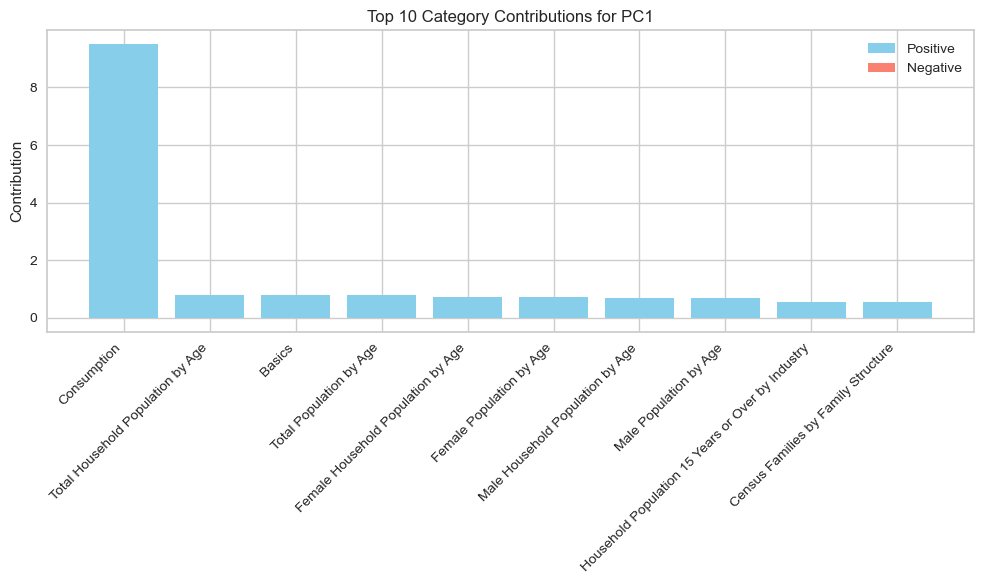
\includegraphics[width=0.9\textwidth]{figures/pc1_contribs.png}
    \caption{Top Contributing Categories to PC1}
    \label{fig:pc1}
\end{figure}

\paragraph{PC2: Immigrant Presence vs. Established Households.}  
PC2 differentiates areas with high immigrant presence from those with more established populations (Figure~\ref{fig:pc2}). While \textit{Consumption} remains a positive factor, the strongest negative contributions come from immigration-related categories such as \textit{Total Immigrants and Place of Birth}, \textit{Period of Immigration}, and \textit{Age at Immigration}. High PC2 scores likely reflect long-established, non-immigrant populations with moderate spending, while lower scores correspond to recent immigrant-dense areas with distinct demographic structures.

\begin{figure}[H]
    \centering
    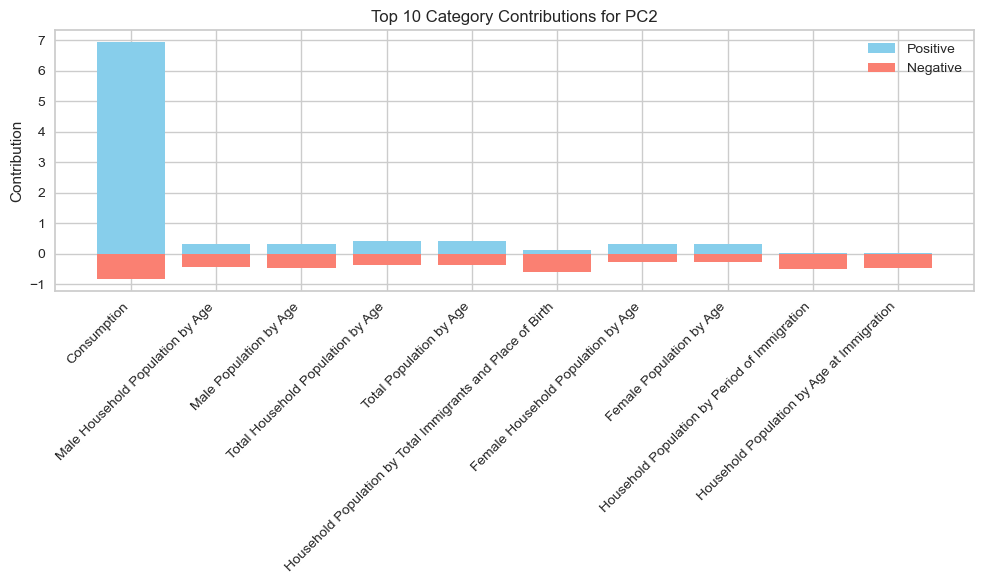
\includegraphics[width=0.9\textwidth]{figures/pc2_contribs.png}
    \caption{Top Contributing Categories to PC2}
    \label{fig:pc2}
\end{figure}

\paragraph{PC3: Household Composition and Structural Living.}  
PC3 seems to reflect differences in household structure and housing type (Figure~\ref{fig:pc3}). Contributions are more muted from \textit{Consumption}, while categories like \textit{Census Family Households by Family Structure}, \textit{Households by Household Type}, and \textit{Occupied Private Dwellings by Structure Type} contribute negatively. This suggests that lower PC3 scores may represent non-traditional or smaller households in denser housing (e.g., apartments), whereas higher scores point to more traditional family units in larger dwellings.

\begin{figure}[H]
    \centering
    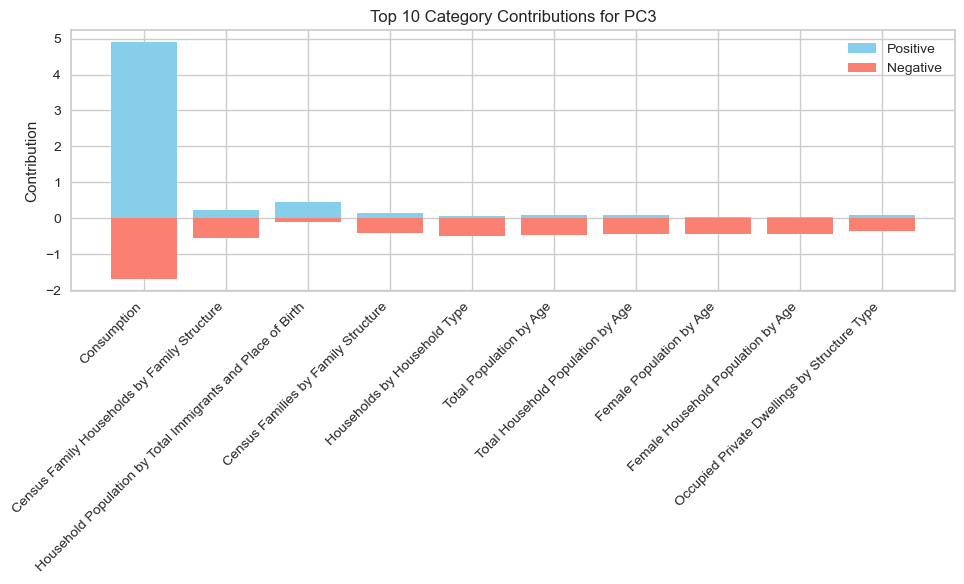
\includegraphics[width=0.9\textwidth]{figures/pc3_contribs.png}
    \caption{Top Contributing Categories to PC3}
    \label{fig:pc3}
\end{figure}

Overall, PCA revealed interpretable latent axes in the data related to economic activity, immigration patterns, and household structure. While clusters in the PCA-projected space are not strongly separable, the broad grouping captured by K-Means aligns with meaningful socioeconomic dimensions.

\paragraph{Cluster Profiling Based on Principal Components}

To better understand the characteristics of the clusters formed by K-Means ($k=3$), we calculated the average values of the first three principal components within each cluster. Since PC1 explains a dominant 67.9\% of the total variance, it serves as the primary basis for interpretation, while PC2 and PC3 (explaining 3.7\% and 3.0\%, respectively) provide additional nuance.

\begin{table}[H]
    \centering
    \caption{Mean Principal Component Scores by Cluster}
    \label{tab:cluster-pc-means}
    \begin{tabular}{@{}cccc@{}}
        \toprule
        Cluster & PC1 Mean & PC2 Mean & PC3 Mean \\
        \midrule
        0 & 37.89 & -0.63 & 0.19 \\
        1 & -15.13 & -0.22 & $\sim$0.00 \\
        2 & 5.19 & 0.80 & -0.11 \\
        \bottomrule
    \end{tabular}
\end{table}

\textbf{Cluster 0: Affluent, Traditional Immigrant Families.}  
This cluster scores highest on PC1, indicating strong consumer activity and dense, demographically diverse households. The slightly negative PC2 score suggests a moderate immigrant presence, while a mildly positive PC3 implies more traditional household structures. These could be higher-income, family-oriented areas with a mix of native and immigrant populations.

\textbf{Cluster 1: Low-Spending, High-Immigration Small Households.}  
Cluster 1 shows the lowest PC1 score, reflecting low household spending and smaller population centers. A modestly negative PC2 indicates relatively recent immigrant populations, and the near-zero PC3 score hints at non-traditional or smaller households. These may represent younger, immigrant-dominated areas with limited consumer capacity and less conventional living arrangements.

\textbf{Cluster 2: Mid-Spending, Native, Non-Traditional Households.}  
This group is moderate on PC1 (spending) and somewhat positive on PC2, suggesting a primarily native-born population. The slightly negative PC3 implies more non-traditional household setups, such as single-person or young professional units, possibly in urban or high-density housing contexts. These areas may be characterized by moderate economic activity and non-family household compositions.

These labels will be used in subsequent visualizations and interpretation.

\subsubsection{Uniform Manifold Approximation and Projection}

\section{Regression}

\appendix
\section*{Appendix}
\section{Extra Silhouette Plots}

\begin{figure}[H]
    \centering
    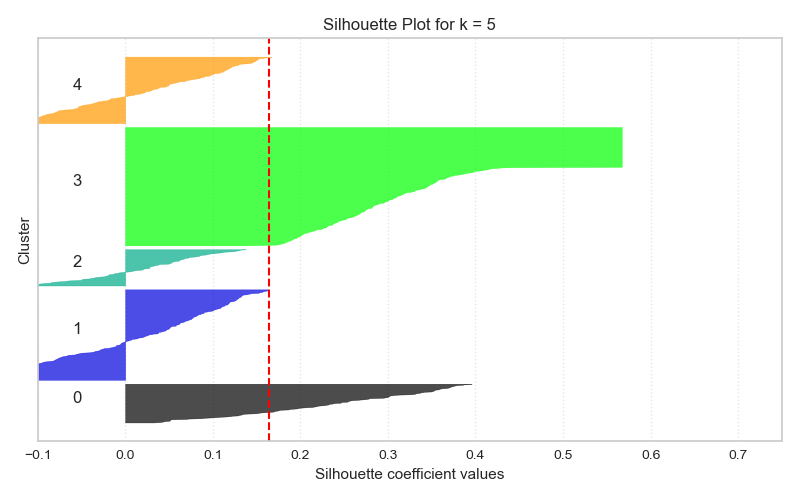
\includegraphics[width=0.6\textwidth]{figures/silhouette_k5.png}
    \caption{Silhouette Plot for $k=5$}
    \label{fig:silhouette_k5}
\end{figure}

\begin{figure}[H]
    \centering
    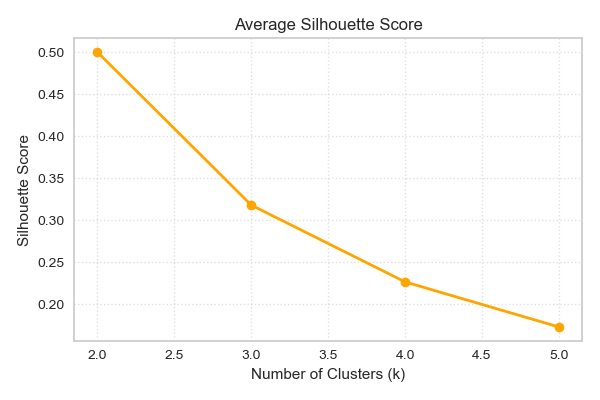
\includegraphics[width=0.65\textwidth]{figures/silhouette_scores.png}
    \caption{Average Silhouette Scores for $k=2$ to $k=5$}
    \label{fig:silhouette_scores}
\end{figure}


\section{PCA Component Loadings}

The following tables show the top five positive and negative variable loadings for each of the first three principal components (PC1–PC3). These values were used to interpret the latent dimensions of the PCA results. HHS refers to the HouseholdSpend dataset.

\begin{table}[H]
\centering
\caption{Top Positive Loadings for PC1}
\label{tab:pc1_pos}
\begin{tabular}{@{}lllll@{}}
\toprule
Variable & HHS Description & HHS Type & DemoStats Category & Loading \\
\midrule
ECYHOMSING & - & - & Language Spoken Most Often At Home & 0.04791 \\
ECYMOTSING & - & - & Mother Tongue & 0.04789 \\
ECYMOBHPOP & - & - & 5-Year Mobility & 0.04789 \\
ECYAIDHPOP & - & - & Indigenous Identity & 0.04788 \\
ECYRIMHPOP & - & - & Recent Immigrants (2017–Present) & 0.04788 \\
\bottomrule
\end{tabular}
\end{table}

\begin{table}[H]
\centering
\caption{Top Negative Loadings for PC1}
\label{tab:pc1_neg}
\begin{tabular}{@{}lllll@{}}
\toprule
Variable & HHS Description & HHS Type & DemoStats Category & Loading \\
\midrule
ECYMTNMED & - & - & Maintainer Age & -0.00437 \\
ECYPFAMED & - & - & Female Population by Age & -0.00413 \\
ECYHFAMED & - & - & Female Household Population by Age & -0.00348 \\
ECYPMAMED & - & - & Male Population by Age & -0.00348 \\
ECYHMAMED & - & - & Male Household Population by Age & -0.00282 \\
\bottomrule
\end{tabular}
\end{table}

\begin{table}[H]
\centering
\caption{Top Positive Loadings for PC2}
\label{tab:pc2_pos}
\begin{tabular}{@{}lllll@{}}
\toprule
Variable & HHS Description & HHS Type & DemoStats Category & Loading \\
\midrule
HSSH037A & Wood/Fuel for Heating & Consumption & - & 0.11518 \\
ECYHTAMED & - & - & Household Pop. by Age & 0.11505 \\
ECYPTAMED & - & - & Total Population by Age & 0.11242 \\
ECYHMAMED & - & - & Male Household Population by Age & 0.10444 \\
HSSH034 & Other Fuel & Consumption & - & 0.10254 \\
\bottomrule
\end{tabular}
\end{table}

\begin{table}[H]
\centering
\caption{Top Negative Loadings for PC2}
\label{tab:pc2_neg}
\begin{tabular}{@{}lllll@{}}
\toprule
Variable & HHS Description & HHS Type & DemoStats Category & Loading \\
\midrule
ECYNCA\_18P & - & - & Citizenship & -0.09457 \\
ECYVISVM & - & - & Visible Minority Status & -0.09315 \\
ECYHOMNOFF & - & - & Language Spoken Most Often At Home & -0.09130 \\
ECYNCANCIT & - & - & Citizenship & -0.09076 \\
ECYPIM1621 & - & - & Period of Immigration & -0.08743 \\
\bottomrule
\end{tabular}
\end{table}

\begin{table}[H]
\centering
\caption{Top Positive Loadings for PC3}
\label{tab:pc3_pos}
\begin{tabular}{@{}lllll@{}}
\toprule
Variable & HHS Description & HHS Type & DemoStats Category & Loading \\
\midrule
HSWH040S & Net Purchase Price of Residences & Consumption & - & 0.13164 \\
HSTE001ZBS & Non-current Consumption & Consumption & - & 0.12020 \\
HSSH033A & Natural Gas (Owned Residence) & Consumption & - & 0.11436 \\
HSSH033 & Natural Gas & Consumption & - & 0.10837 \\
ECYCHAHHCH & - & - & Children at Home by Age & 0.10319 \\
\bottomrule
\end{tabular}
\end{table}

\begin{table}[H]
\centering
\caption{Top Negative Loadings for PC3}
\label{tab:pc3_neg}
\begin{tabular}{@{}lllll@{}}
\toprule
Variable & HHS Description & HHS Type & DemoStats Category & Loading \\
\midrule
ECYSTYAPU5 & - & - & Structure Type & -0.13074 \\
ECYMOTFREN & - & - & Mother Tongue & -0.12838 \\
ECYSTYAPT & - & - & Structure Type & -0.12515 \\
ECYHOMFREN & - & - & Language Spoken Most Often At Home & -0.12314 \\
\bottomrule
\end{tabular}
\end{table}


\end{document}